\chapter{Resultados}\label{cap:resultados}

\section{Influência dos Parâmetros no Comportamento do Time}

Nesta secção são apresentados os diferentes comportamentos
que podem ser obtidos através da modificação dos parâmetros
apresentados no capítulo~\ref{cap:modelagem}. Cada parâmetro
é modificado e os resultados na mudança do planejamento são
evidenciados.

Os parâmetros iniciais são definidos no arquivo src/consts.h, % TODO: referenciar anexos
cujos valores são:

% TODO: Substituir nomes das variáveis, conforme a modelagem
\begin{itemize}
  \item $CONSTANT{\_}RATE = true$
  \item $KICK{\_}IF{\_}NO{\_}PASS = false$
  \item $DECISION{\_}RATE = 7$
  \item $RAMIFICATION{\_}NUMBER = 5000$
  \item $FULL{\_}CHANGE{\_}PERCENTAGE = 100$
  \item $MAX{\_}DEPTH = 0$
  \item $KICK{\_}POS{\_}VARIATION = 0.150$
  \item $MIN{\_}GAP{\_}TO{\_}KICK = 18.0$
  \item $DESIRED{\_}PASS{\_}DIST = 2.0$
  \item $WEIGHT{\_}BALL{\_}POS = 0$
  \item $WEIGHT{\_}MOVE{\_}DIST{\_}MAX = 0$
  \item $WEIGHT{\_}MOVE{\_}DIST{\_}TOTAL = 0$
  \item $WEIGHT{\_}MOVE{\_}CHANGE = 2$
  \item $WEIGHT{\_}PASS{\_}CHANGE = 2$
  \item $WEIGHT{\_}KICK{\_}CHANGE = 2$
  \item $TOTAL{\_}MAX{\_}GAP{\_}RATIO = 0.5$
  \item $WEIGHT{\_}CLOSE{\_}TO{\_}BALL = 1000$
  \item $WEIGHT{\_}ENEMY{\_}CLOSE{\_}TO{\_}BALL = 1000$
  \item $WEIGHT{\_}HAS{\_}BALL = 5000$
  \item $WEIGHT{\_}ATTACK = 1000$
  \item $WEIGHT{\_}SEE{\_}ENEMY{\_}GOAL = 10$
  \item $WEIGHT{\_}BLOCK{\_}GOAL = 180$
  \item $WEIGHT{\_}BLOCK{\_}ATTACKER = 5000$
  \item $WEIGHT{\_}GOOD{\_}RECEIVERS = 0$
  \item $WEIGHT{\_}RECEIVERS{\_}NUM = 20$
  \item $WEIGHT{\_}ENEMY{\_}RECEIVERS{\_}NUM = 20$
  \item $DIST{\_}GOAL{\_}PENAL = 2000$
  \item $DIST{\_}GOAL{\_}TO{\_}PENAL = 1.0$
  \item $MOVE{\_}RADIUS{\_}0 = 0.5$
  \item $MOVE{\_}RADIUS{\_}1 = 2.0$
  \item $MOVE{\_}RADIUS{\_}2 = 7.0$
\end{itemize}

A figura~\ref{fig:default} apresenta o planejamento em um
ambiente de ataque e defesa com os parâmetros iniciais
apresentados anteriormente.

\begin{figure}
  \centering
  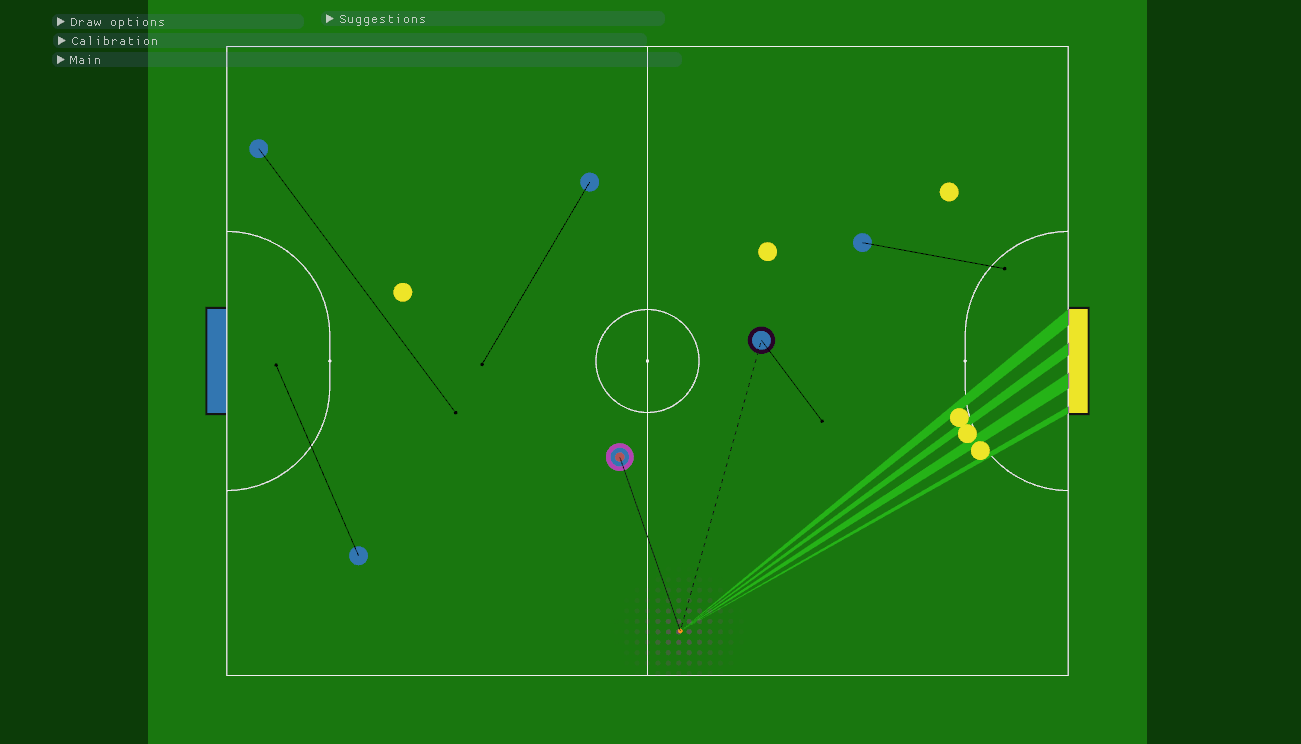
\includegraphics[width= 0.8\linewidth]{result/default_atq}
  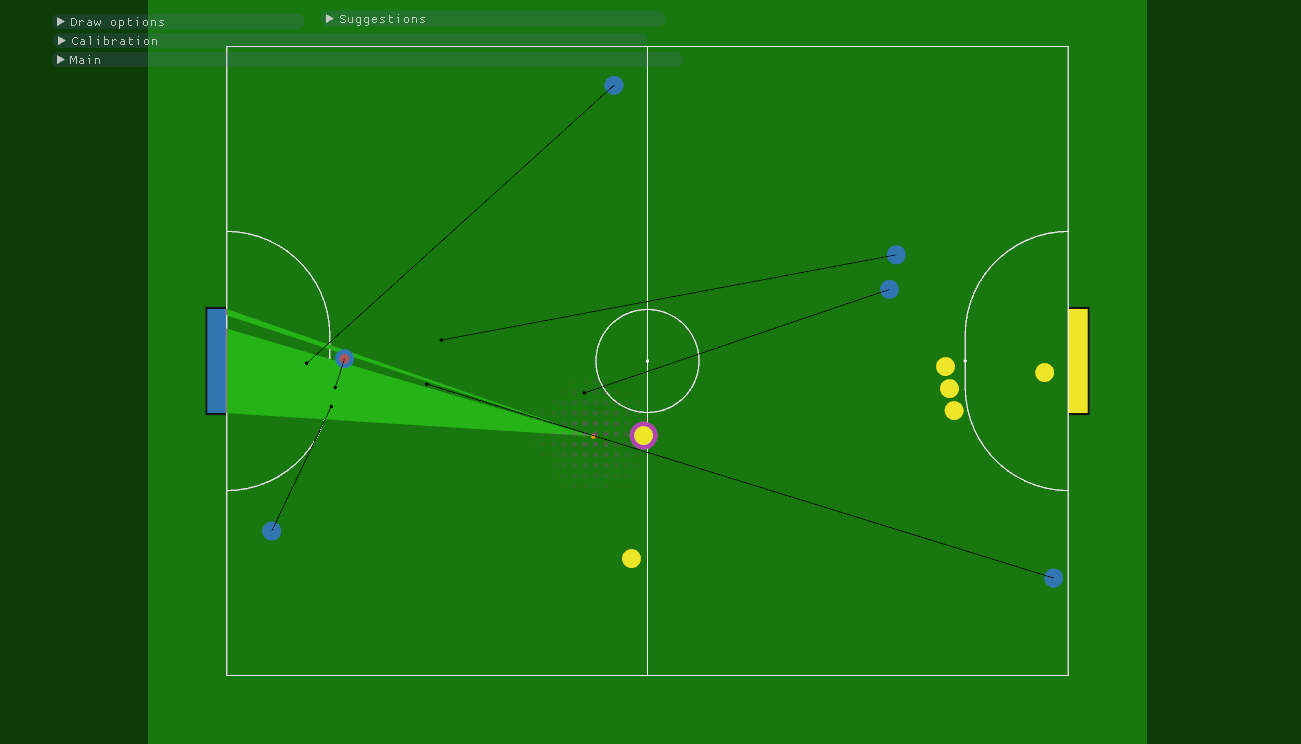
\includegraphics[width= 0.8\linewidth]{result/default_def}
  \caption{Planejamento com os parâmetros iniciais no
           ataque (acima) e na defesa (abaixo)}\label{fig:default}
\end{figure}

\subsection{Correção da Abertura do Gol Devido a Movimentação da Bola}

Somente o ajuste de movimentação da bola foi anulado. Os resultados
no planejamento são apresentados na Figura~\ref{fig:kickpos_0}.
Conforme pode ser observado, a sombra dos robôs é maior, reduzindo
assim abertura do gol. Logo, poucos robôs são necessários
para bloquear o gol. Isso gerou mais ações direcionadas para posições
de ataque.

\begin{figure}[H]
  \centering
  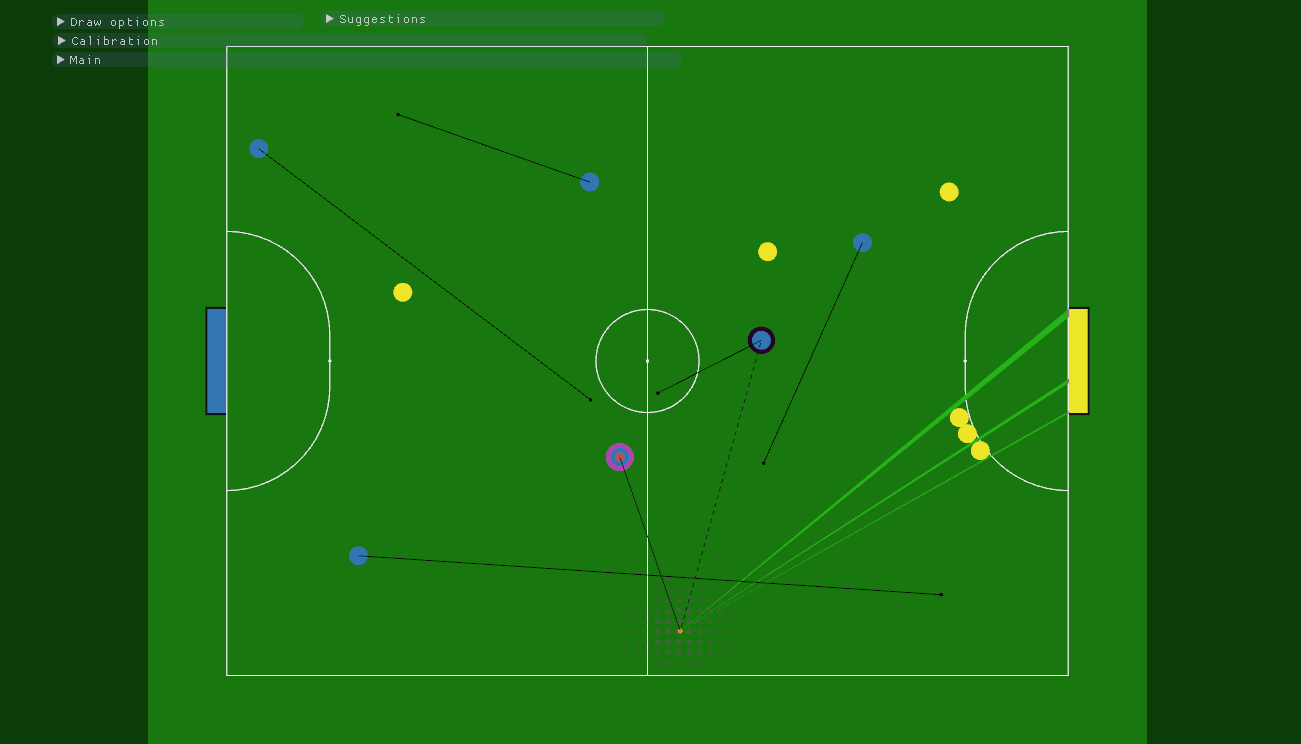
\includegraphics[width= 0.8\linewidth]{result/kickpos_0_atq}
  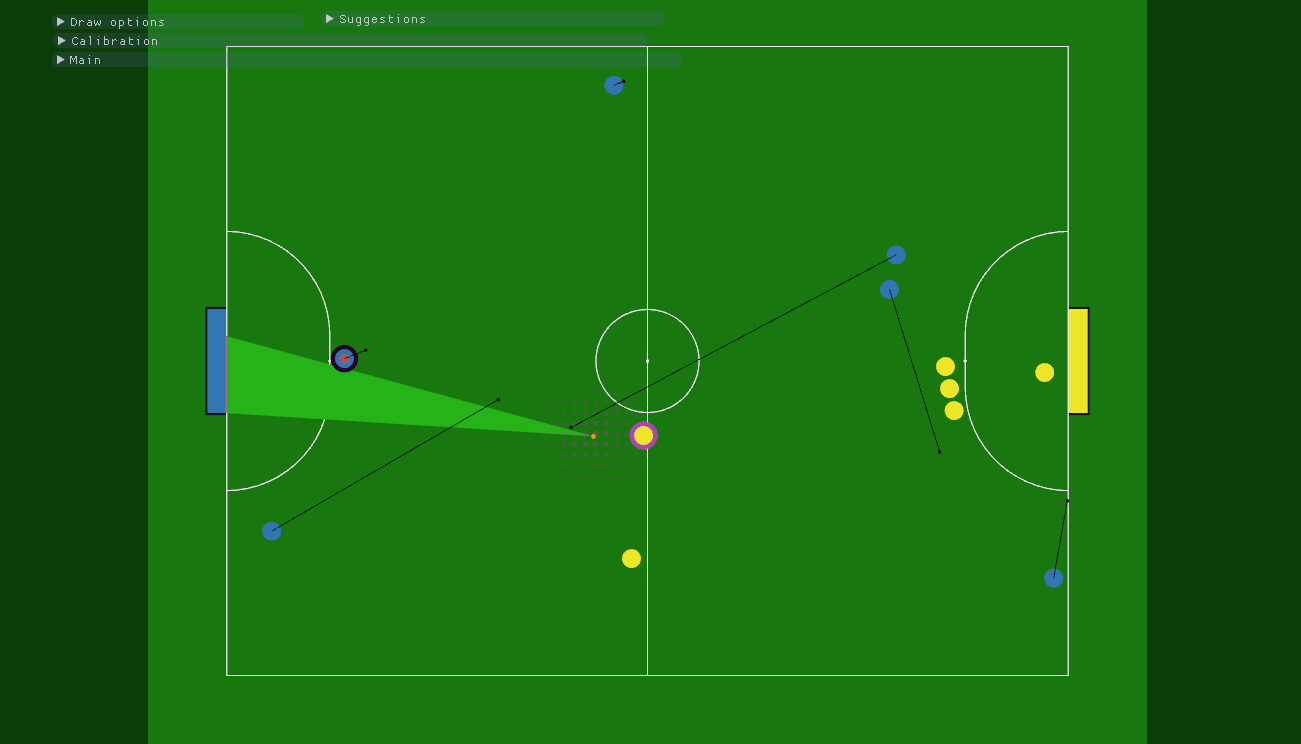
\includegraphics[width= 0.8\linewidth]{result/kickpos_0_def}
  \caption{Planejamento com os parâmetros inicias e sem ajuste
           de movimentação da bola em ambiente de
           ataque (acima) e defesa (abaixo)}\label{fig:kickpos_0}
\end{figure}

Depois esse ajuste foi alterado para $0.24$. Os resultados 
em ambiente de ataque e defesa são apresentados na
Figura~\ref{fig:kickpos_024}. A sombra de cada robô é
menor, resultando em mais robôs próximos ao gol para
reduzir a abertura do gol vista pelos robôs adversários.

\begin{figure}[H]
  \centering
  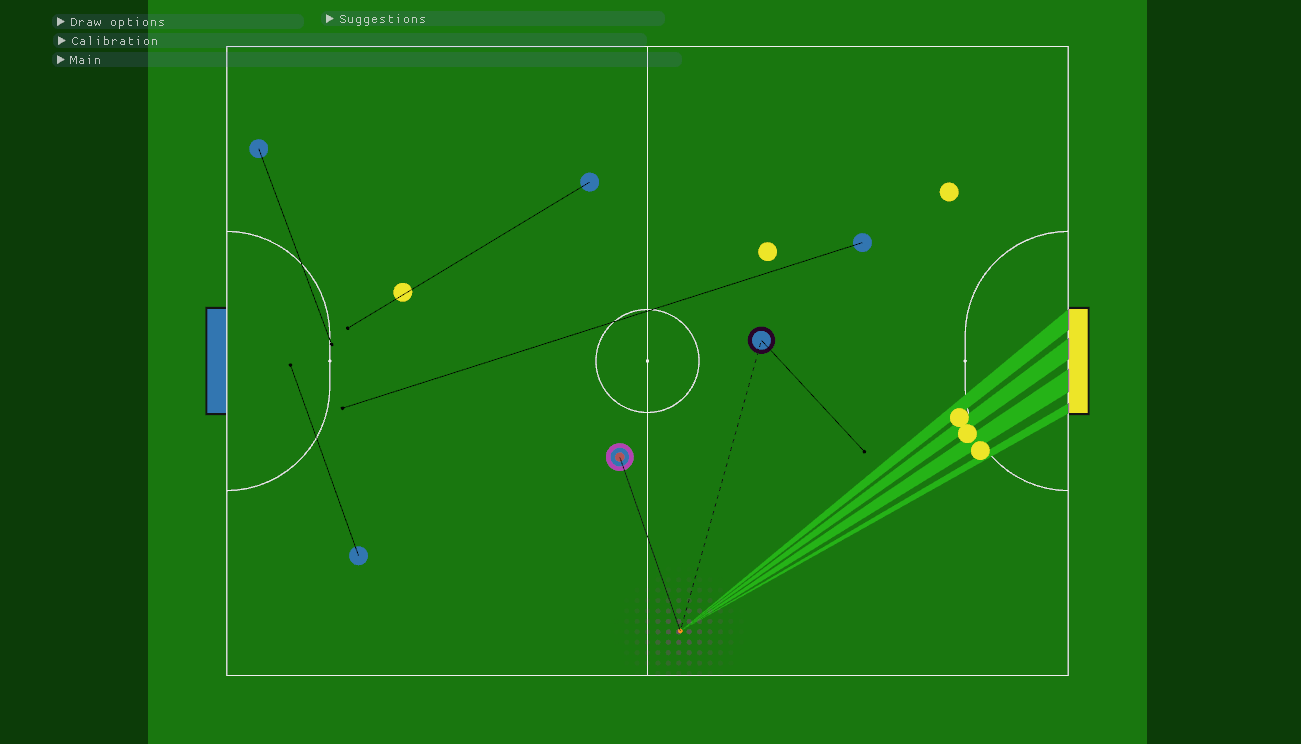
\includegraphics[width= 0.8\linewidth]{result/kickpos_024_atq}
  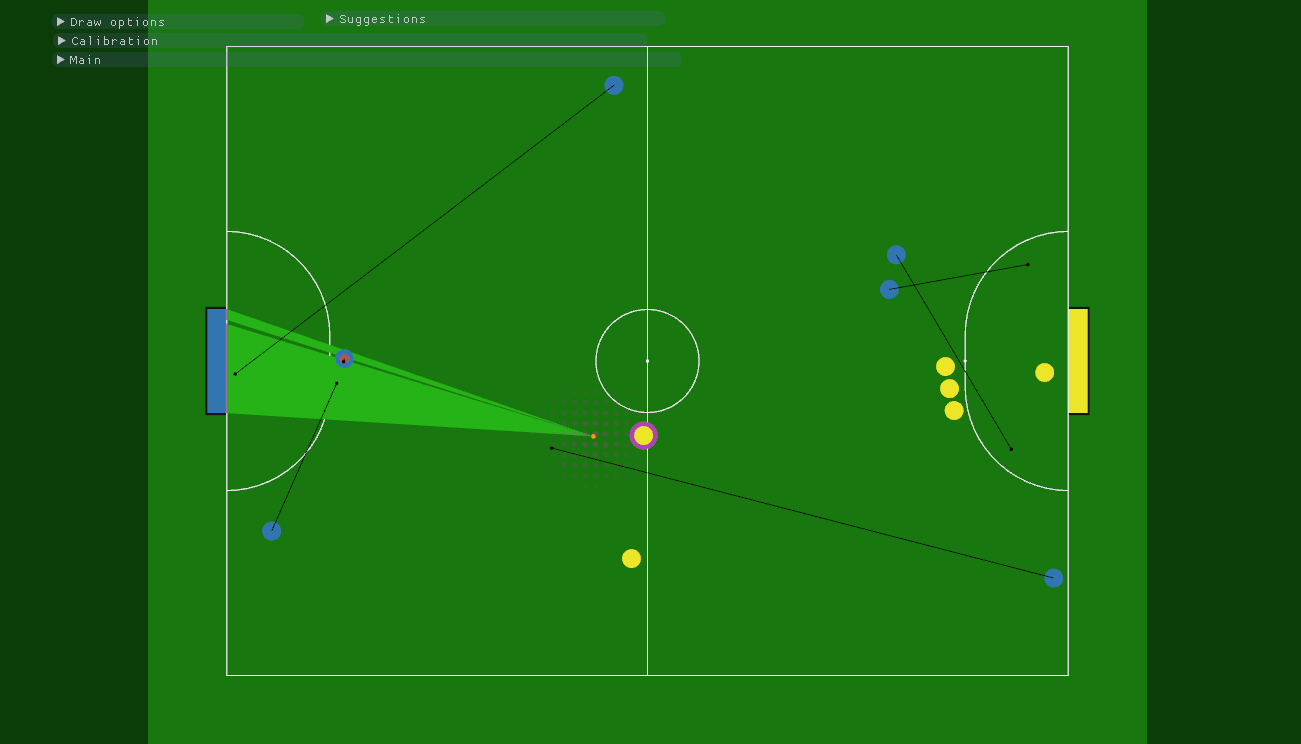
\includegraphics[width= 0.8\linewidth]{result/kickpos_024_def}
  \caption{Planejamento com os parâmetros inicias e o ajuste de
           movimentação da bola ajustado para $0.24$ em ambiente de
           ataque (acima) e defesa (abaixo)}\label{fig:kickpos_024}
\end{figure}

\subsection{Distância Total dos Moves}

Somente o peso do custo da distância total dos moves foi alterado para $10$. Os
resultados no planejamento são apresentados na
Figura~\ref{fig:mov_dist_total_10}.

\begin{figure}[H]
  \centering
  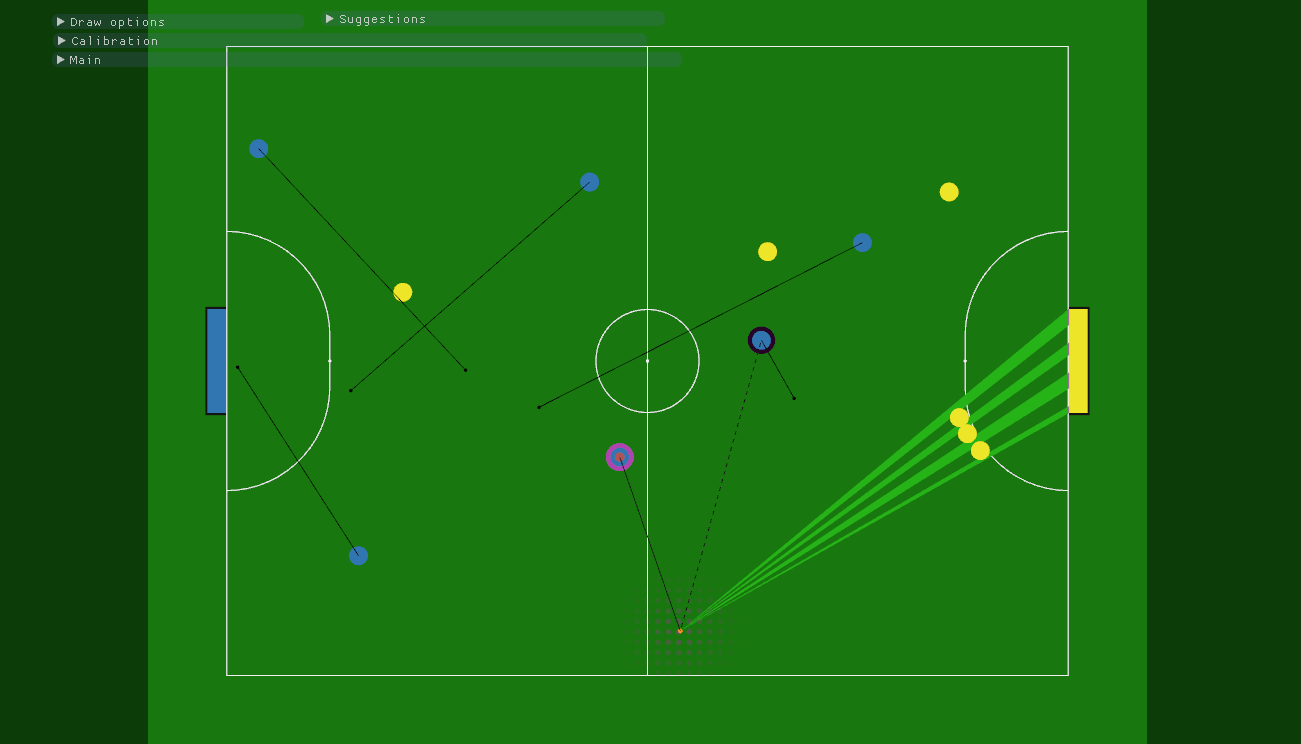
\includegraphics[width= 0.8\linewidth]{result/mov_dist_total_atq_10}
  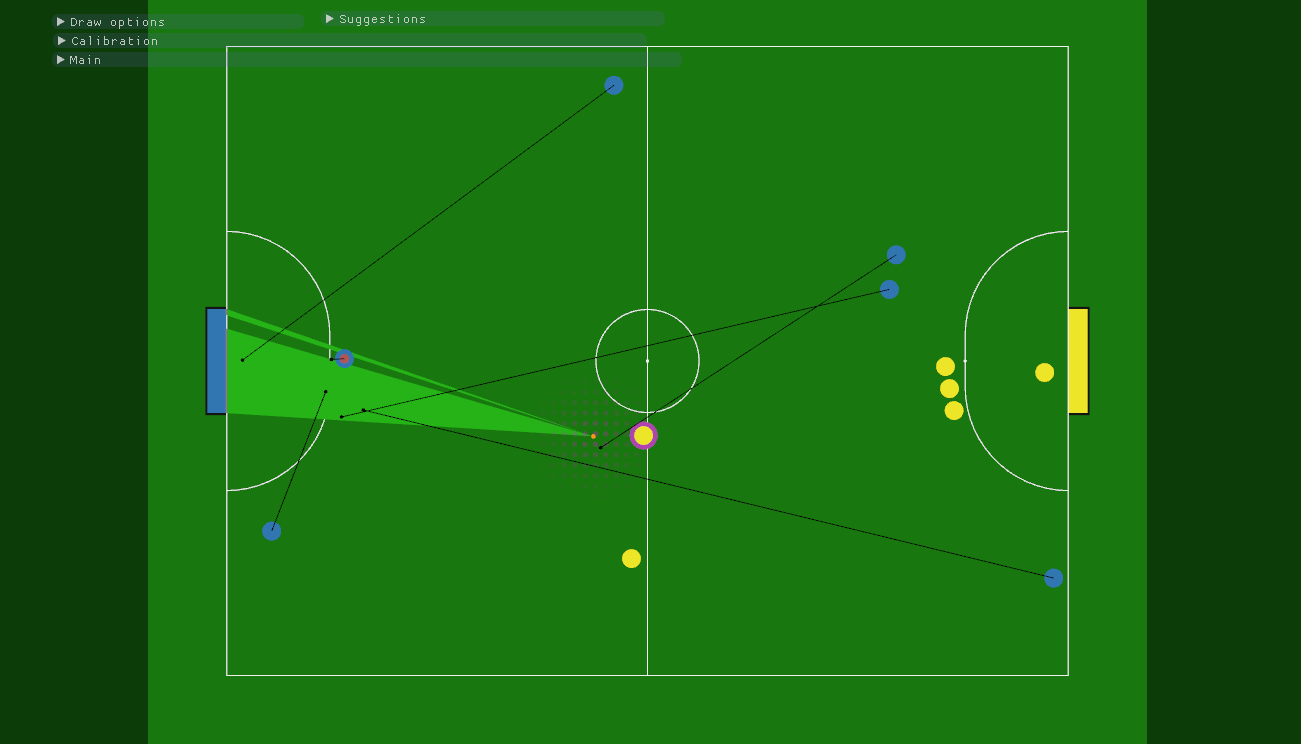
\includegraphics[width= 0.8\linewidth]{result/mov_dist_total_def_10}
  \caption{Planejamento com os parâmetros iniciais e o peso do custo da
  distância total dos moves alterado para $10$.  Ataque (acima) e na defesa (abaixo)}\label{fig:mov_dist_total_10}
\end{figure}

% vim: tw=80 et ts=2 sw=2 sts=2 ft=tex

\subsection{Distância Máxima dos Moves} 
Somente o peso do custo da distância máxima dos moves foi
alterado para $10$. Os resultados no planejamento são
apresentados na figura~\ref{fig:mov_dist_max_10}.

\begin{figure}[H]
  \centering
  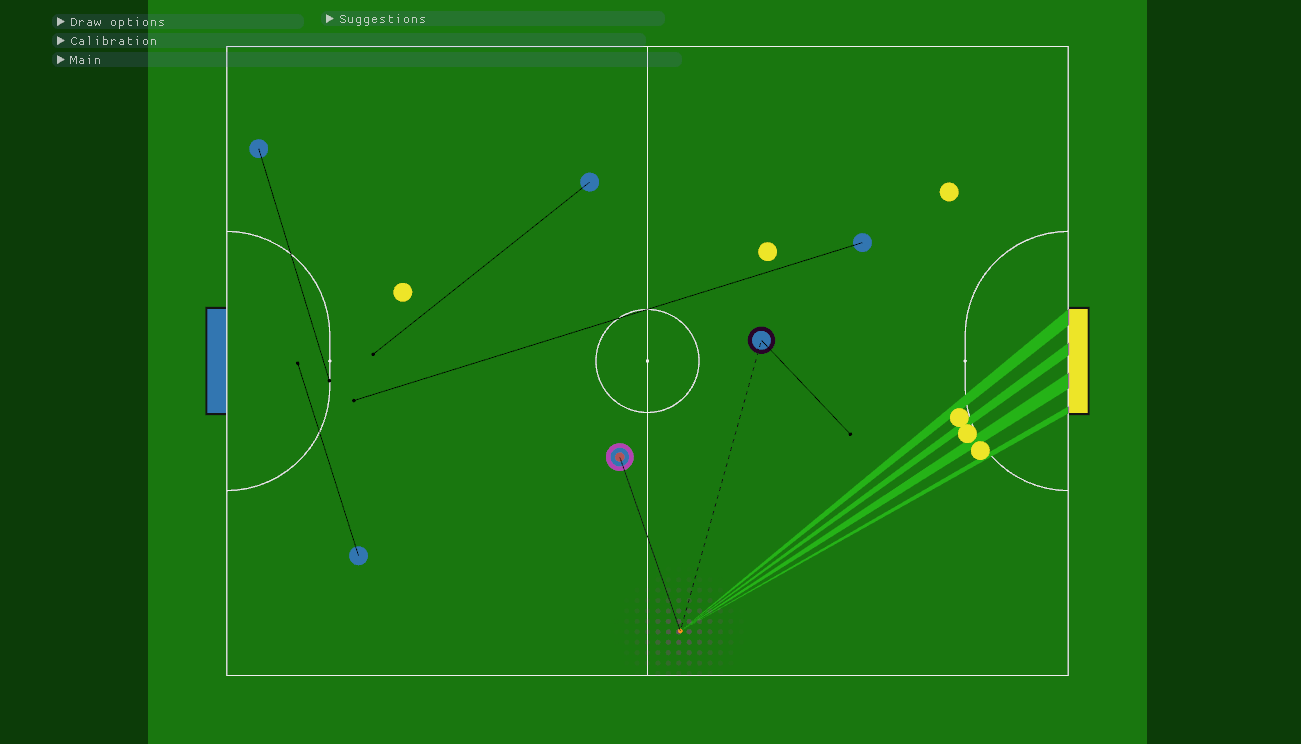
\includegraphics[width= 0.8\linewidth]{result/mov_dist_max_atq_10}
  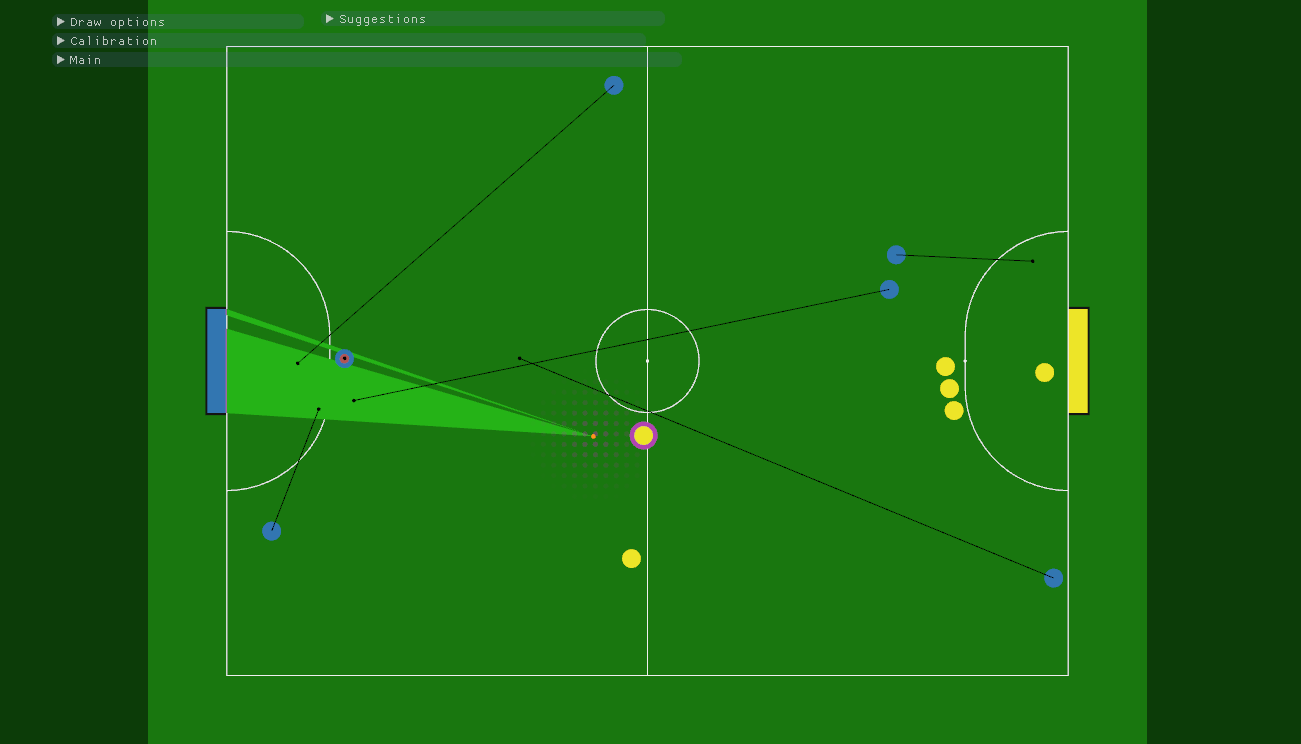
\includegraphics[width= 0.8\linewidth]{result/mov_dist_max_def_10}
  \caption{Planejamento com os parâmetros iniciais e o peso do
           custo da distância máxima dos moves alterado para $10$.
           Ataque (acima) e na defesa (abaixo)}\label{fig:mov_dist_max_10}
\end{figure}

\subsection{Custo do Ataque}
Somente o peso do custo do ataque foi alterado para $5000$.
Os resultados no planejamento são apresentados na
figura~\ref{fig:atack_5000}.

\begin{figure}[H]
  \centering
  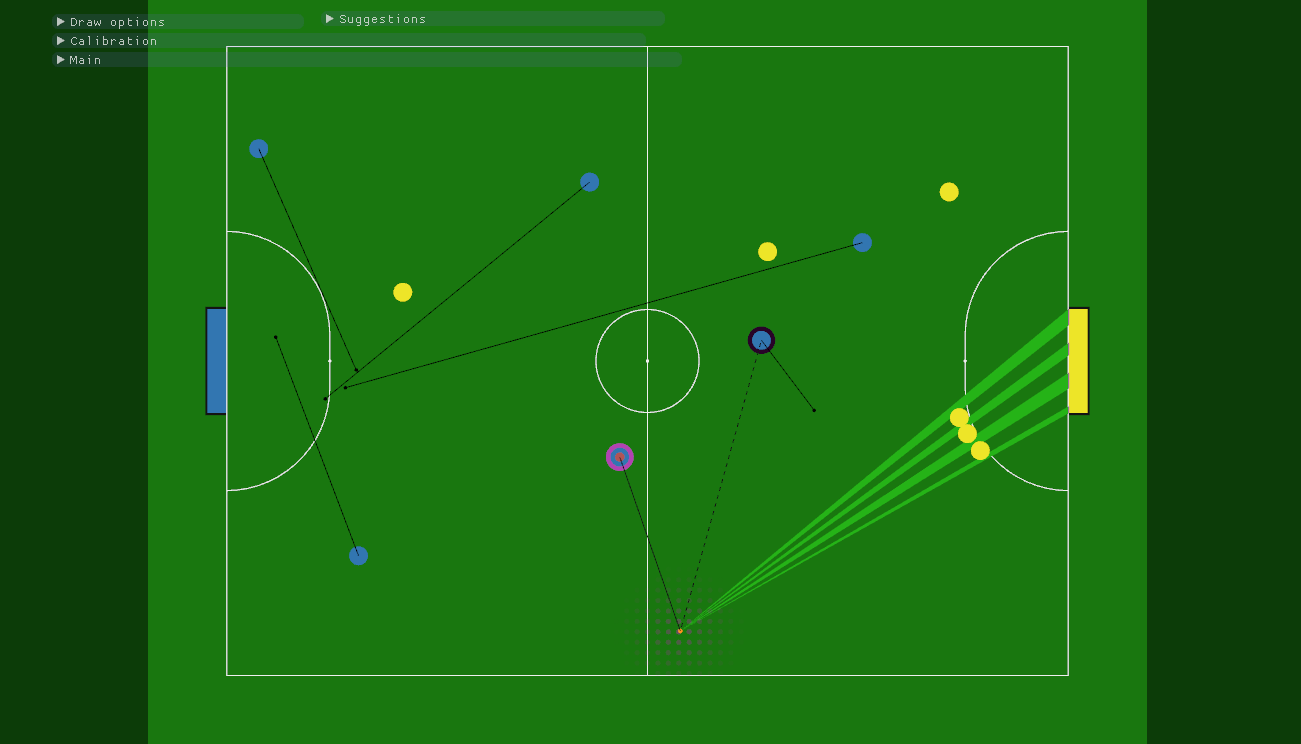
\includegraphics[width= 0.8\linewidth]{result/atack_atq_5000}
  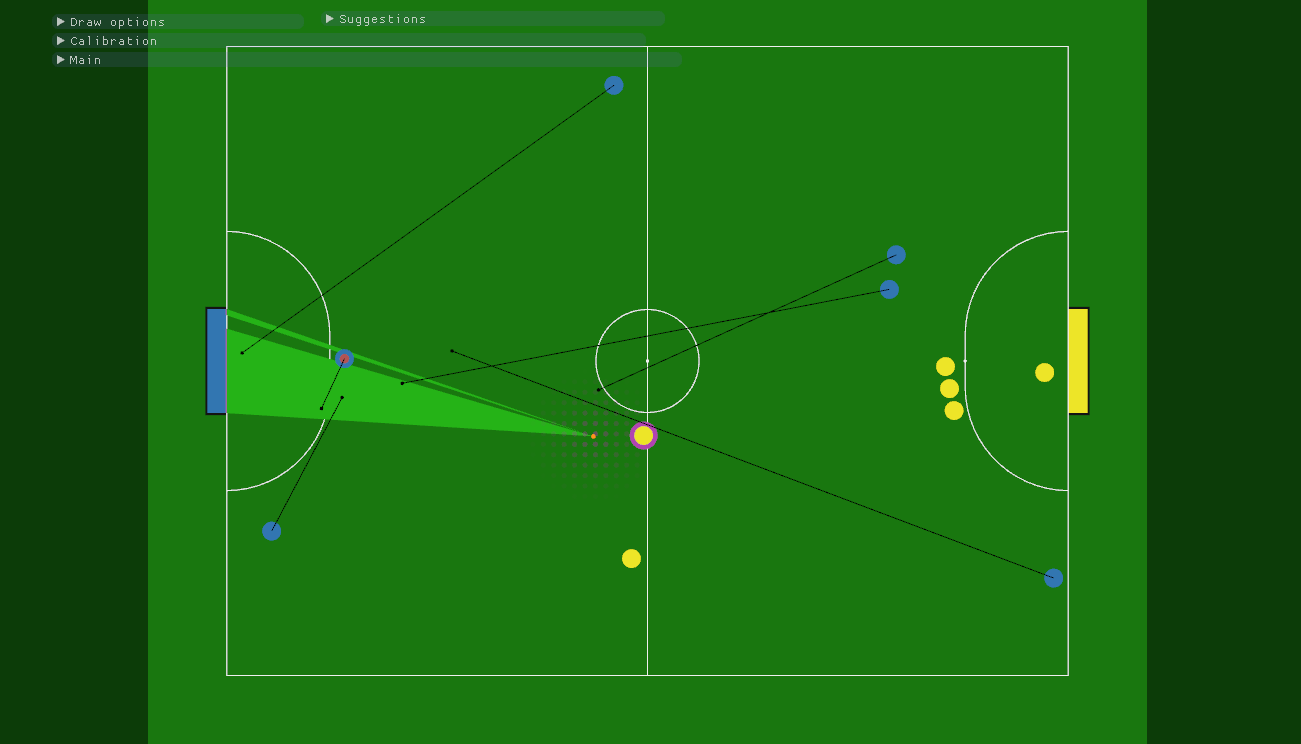
\includegraphics[width= 0.8\linewidth]{result/atack_def_5000}
  \caption{Planejamento com os parâmetros iniciais e o peso do
           custo do ataque alterado para $5000$.
           No ataque (acima) e na defesa (abaixo)}\label{fig:atack_5000}
\end{figure}

\subsection{Custo da Defesa}
% TODO

\begin{figure}[H]
  \centering
  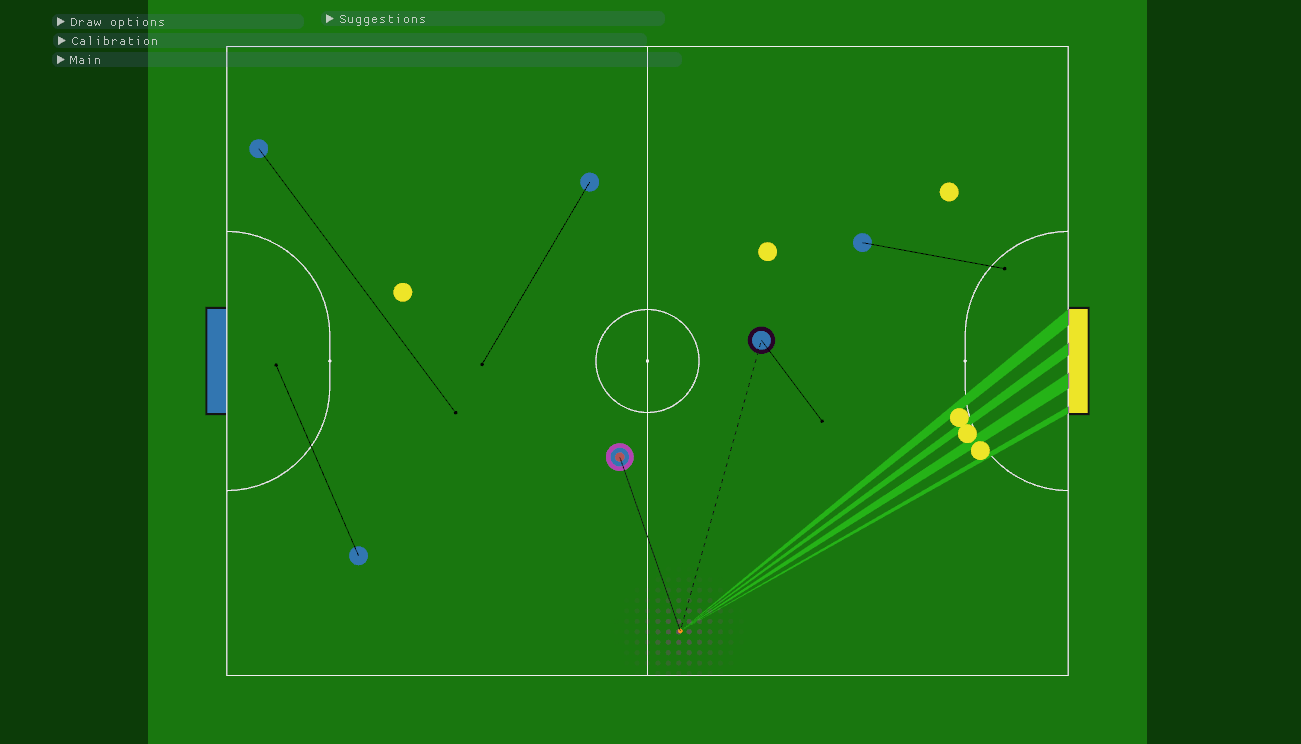
\includegraphics[width= 0.8\linewidth]{result/default_atq}
  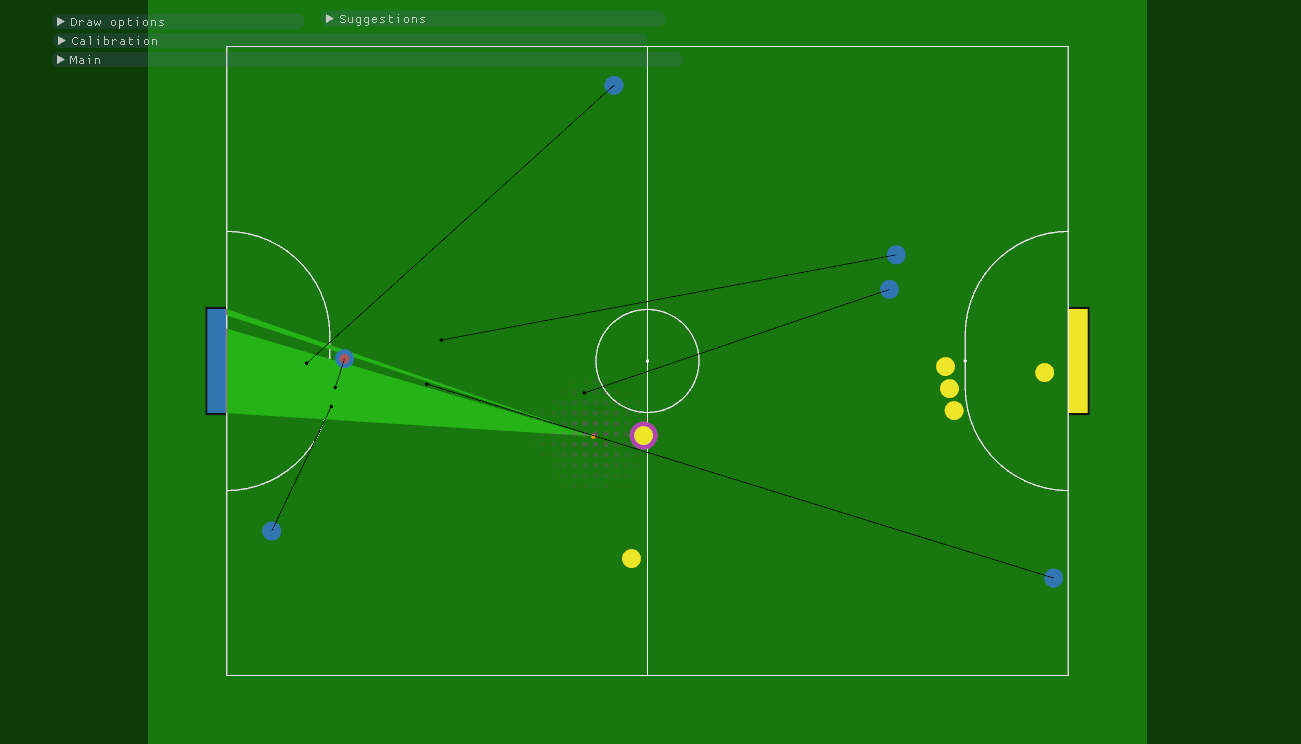
\includegraphics[width= 0.8\linewidth]{result/default_def}
  \caption{Planejamento com os parâmetros iniciais no
           ataque (acima) e na defesa (abaixo)}\label{fig:default}
\end{figure}

\subsection{Mudança do Planejamento da Move Table}
% TODO

\begin{figure}[H]
  \centering
  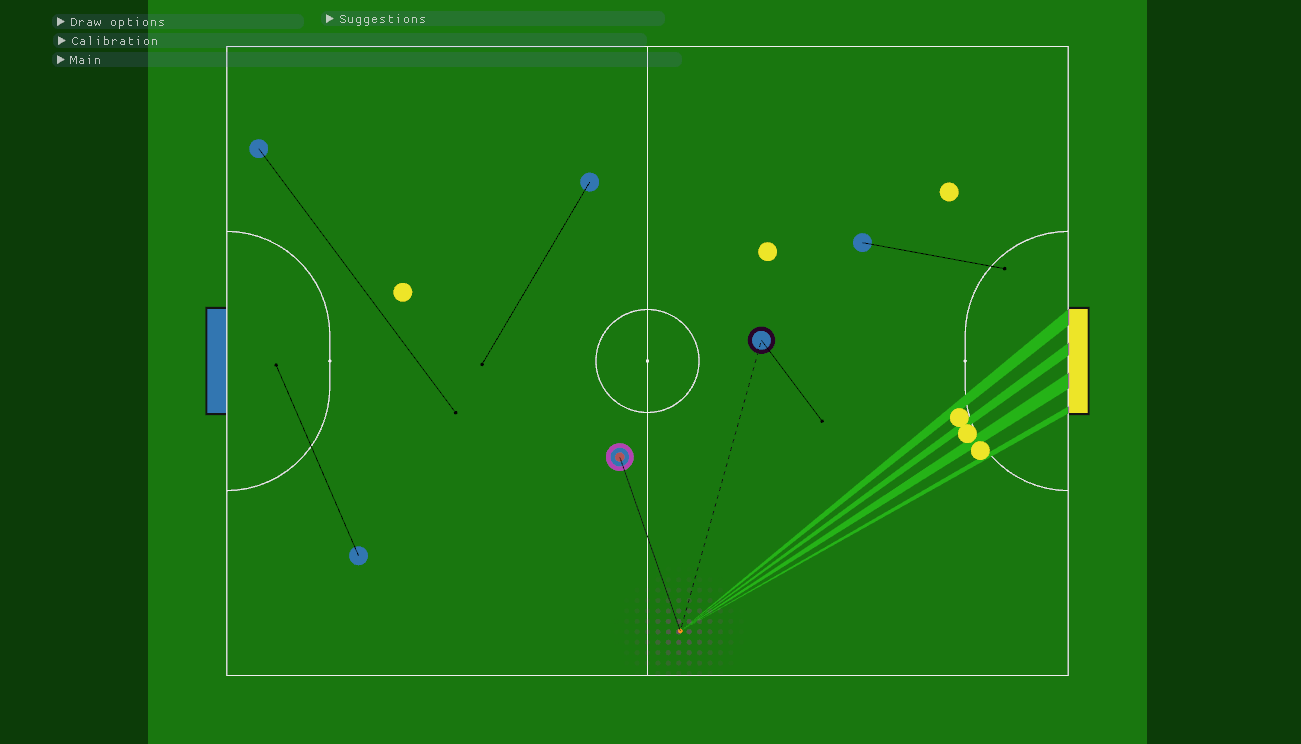
\includegraphics[width= 0.8\linewidth]{result/default_atq}
  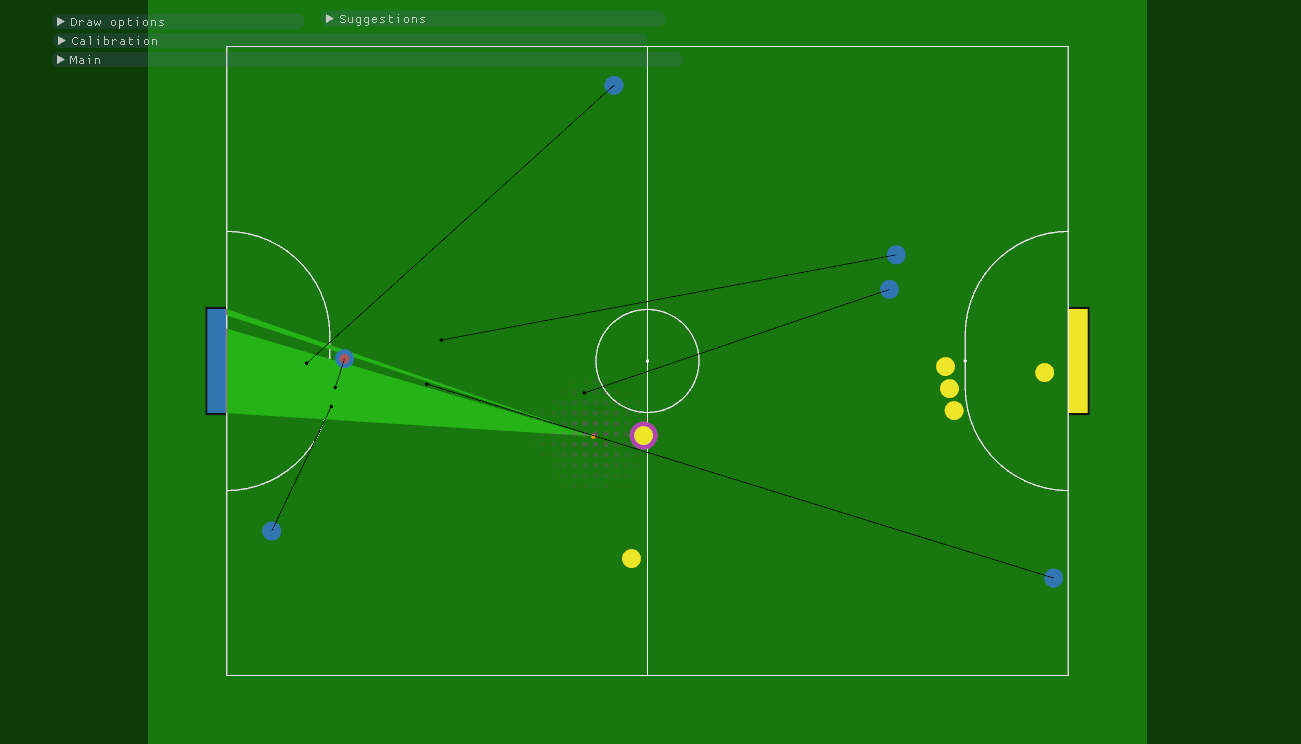
\includegraphics[width= 0.8\linewidth]{result/default_def}
  \caption{Planejamento com os parâmetros iniciais no
           ataque (acima) e na defesa (abaixo)}\label{fig:default}
\end{figure}

\subsection{Custo das Aberturas vistas por $r \in T_c$}

Somente o peso do custo das aberturas do gol vistas pelos robôs do time foi
alterado para $1000$. Os resultados no planejamento são apresentados na
Figura~\ref{fig:see_enemy_goal_1000}. Fica evidente em ambos os ambientes de
ataque e defesa que os robôs se posicionaram o mais próximo possível do gol de
$T_{ad}$, se limitando apenas pela penalização por proximidade do gol
adversário.

\begin{figure}[H]
  \centering
  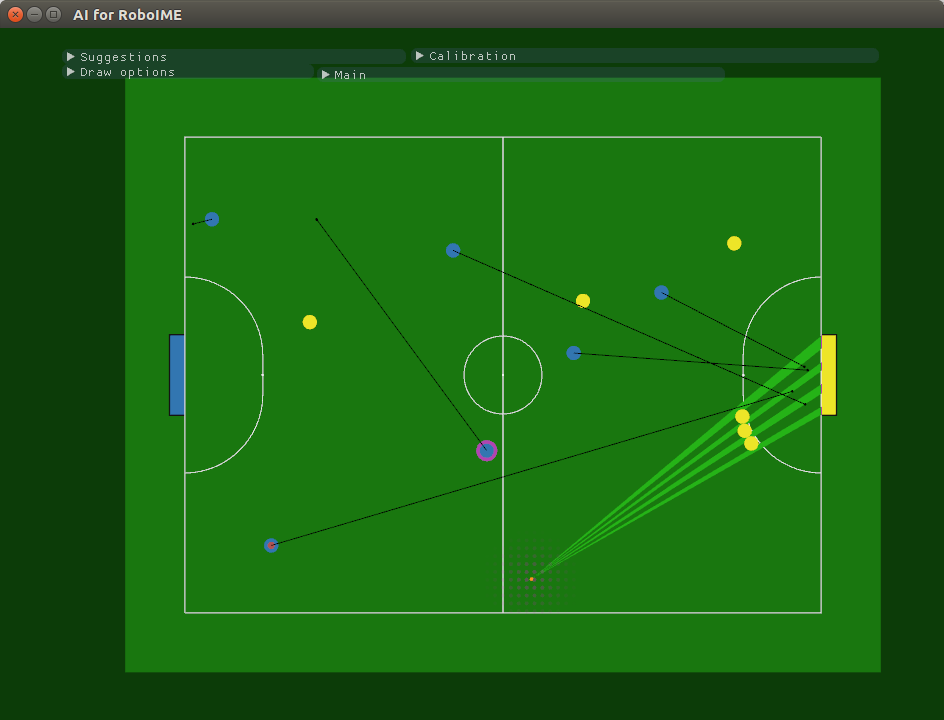
\includegraphics[width= 0.8\linewidth]{result/see_enemy_goal_atq_1000}
  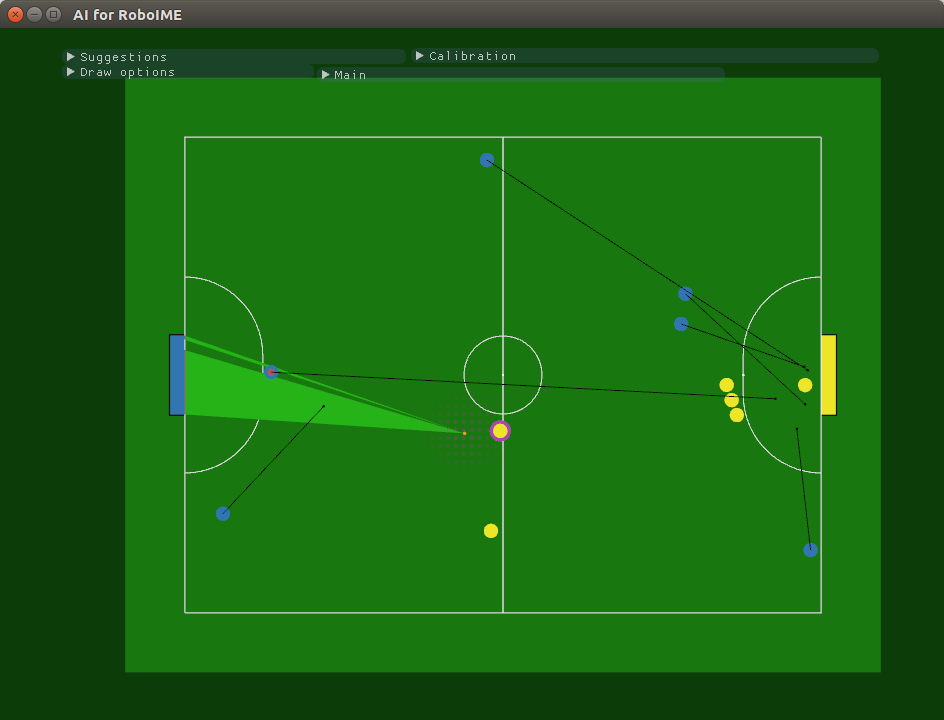
\includegraphics[width= 0.8\linewidth]{result/see_enemy_goal_def_1000}
  \caption{Planejamento com os parâmetros iniciais e com o peso do custo das
  aberturas do gol vistas pelos robôs do time igual a $1000$.  No ataque (acima)
  e na defesa (abaixo)}\label{fig:see_enemy_goal_1000}
\end{figure}

% vim: tw=80 et ts=2 sw=2 sts=2 ft=tex

\subsection{Custo das Aberturas vistas por $r \in T_{ad}$}
Somente o peso do custo das aberturas do goal vistas pelos robôs do time
adversário alterado para zero. Os resultados no planejamento são
apresentados na Figura~\ref{fig:block_goal_0}. Houve uma redução nas
posições de defesa com e sem posse de bola.

\begin{figure}[H]
  \centering
  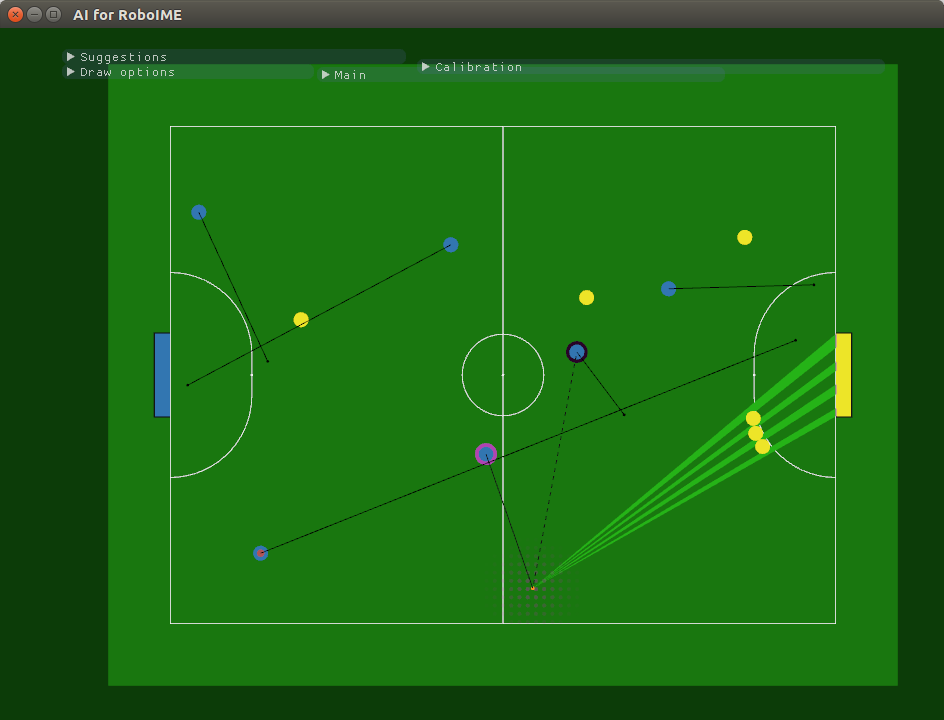
\includegraphics[width= 0.8\linewidth]{result/block_goal_atq_0}
  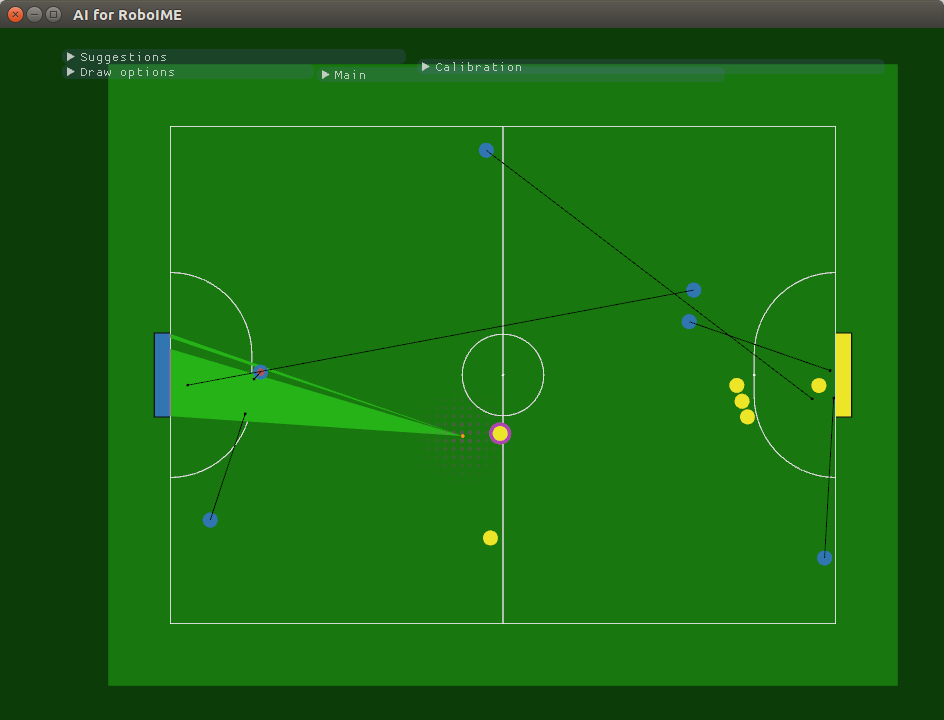
\includegraphics[width= 0.8\linewidth]{result/block_goal_def_0}
  \caption{Planejamento com os parâmetros iniciais e com o custo
           das aberturas do goal vistos pelos robôs do time nulo.
           No ataque (acima) e na defesa (abaixo)}\label{fig:block_goal_0}
\end{figure}

\subsection{Número de Receptores}
% TODO

\begin{figure}[H]
  \centering
  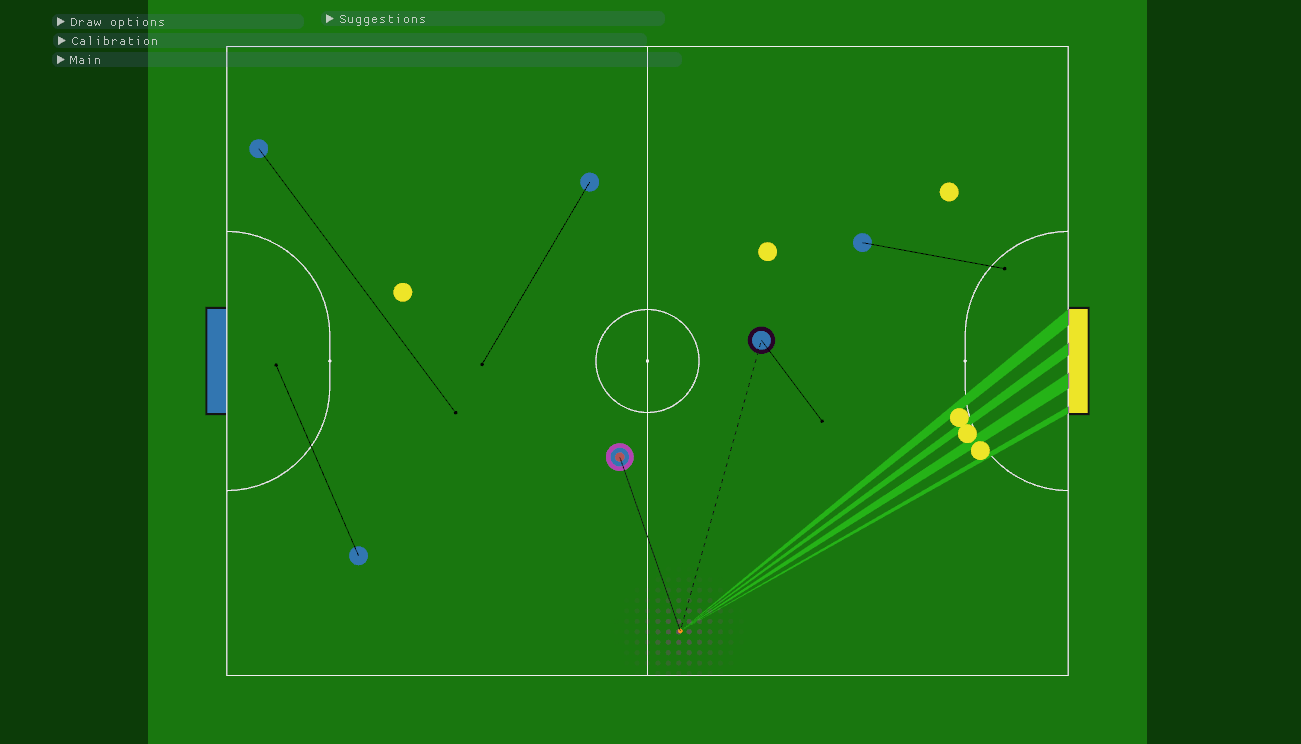
\includegraphics[width= 0.8\linewidth]{result/default_atq}
  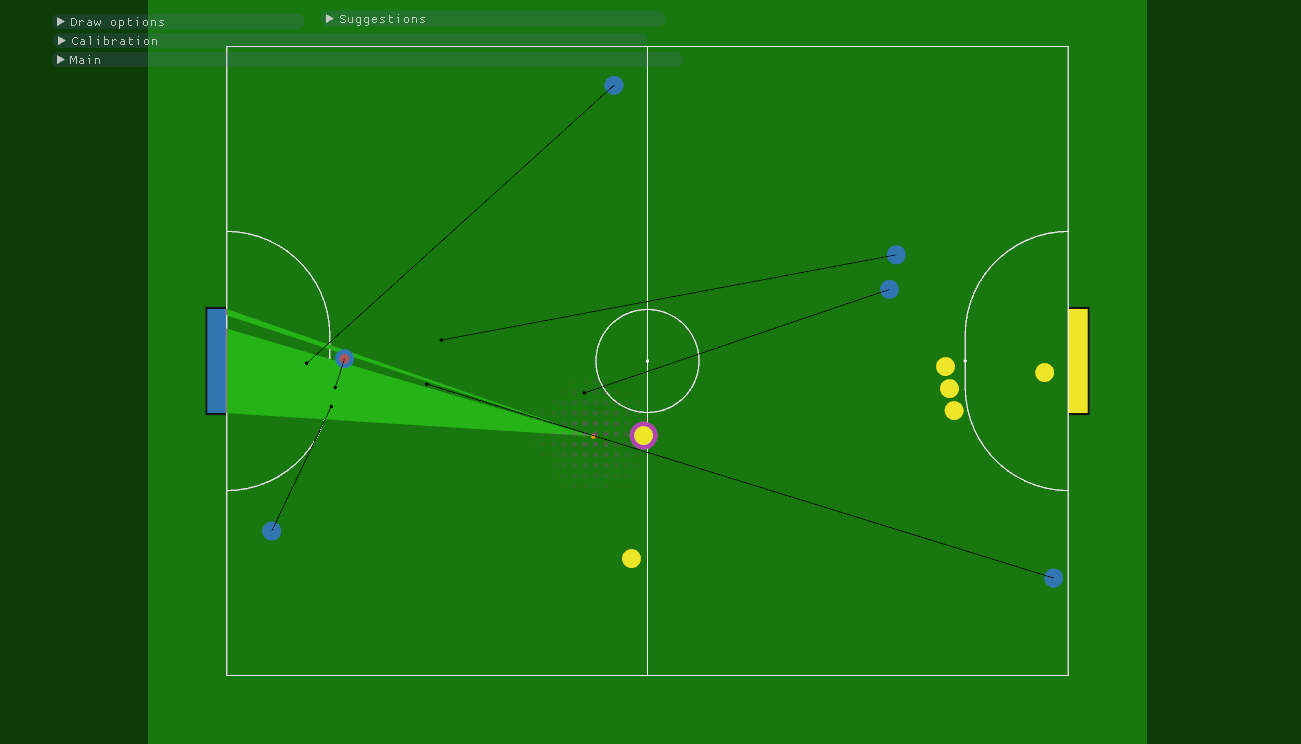
\includegraphics[width= 0.8\linewidth]{result/default_def}
  \caption{Planejamento com os parâmetros iniciais no
           ataque (acima) e na defesa (abaixo)}\label{fig:default}
\end{figure}

\subsection{Penalização por proximidade}
% TODO

\begin{figure}[H]
  \centering
  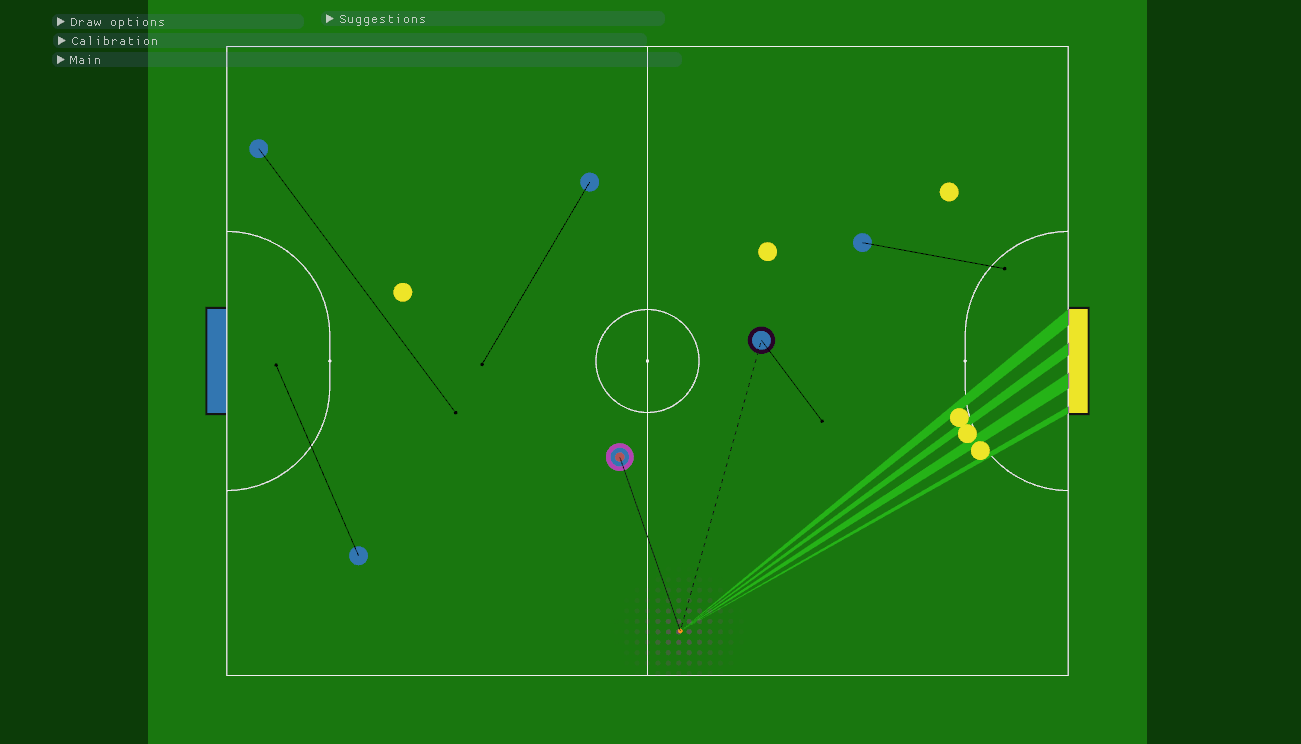
\includegraphics[width= 0.8\linewidth]{result/default_atq}
  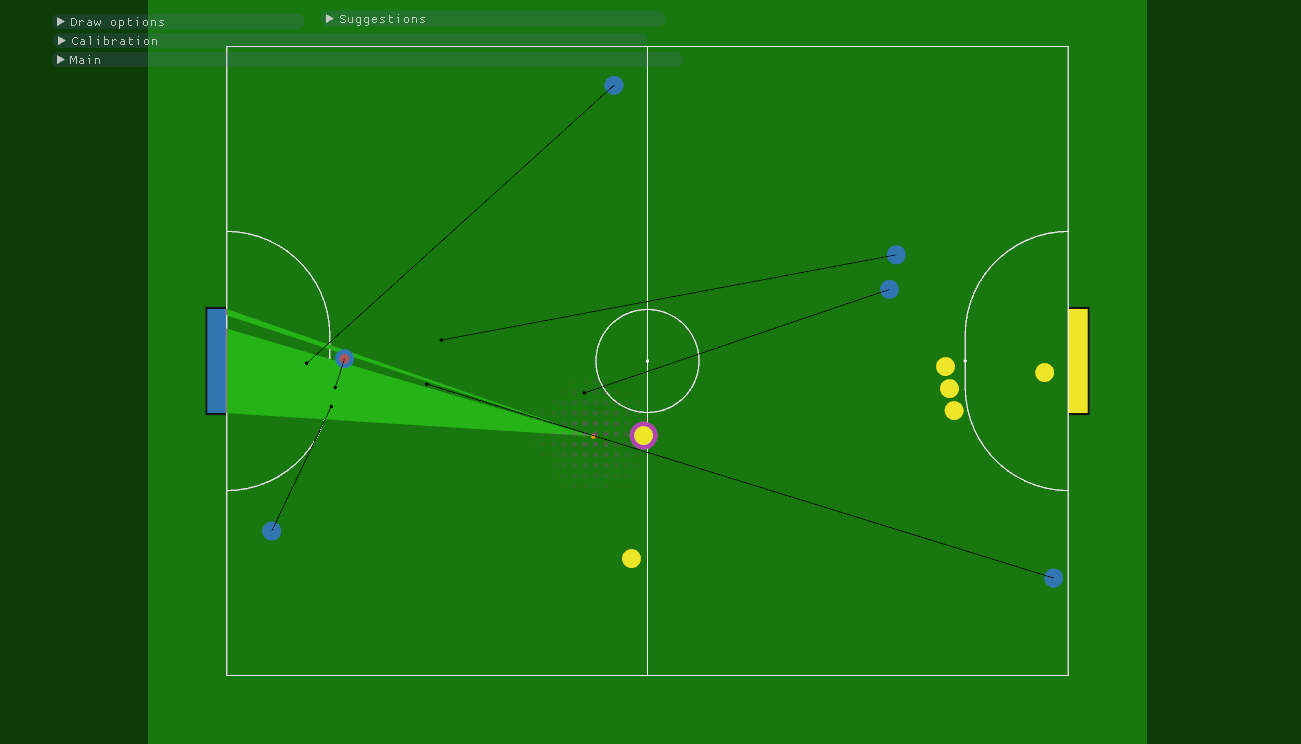
\includegraphics[width= 0.8\linewidth]{result/default_def}
  \caption{Planejamento com os parâmetros iniciais no
           ataque (acima) e na defesa (abaixo)}\label{fig:default}
\end{figure}

\subsection{Penalização por próximidade do gol do adversário}
% TODO

\begin{figure}[H]
  \centering
  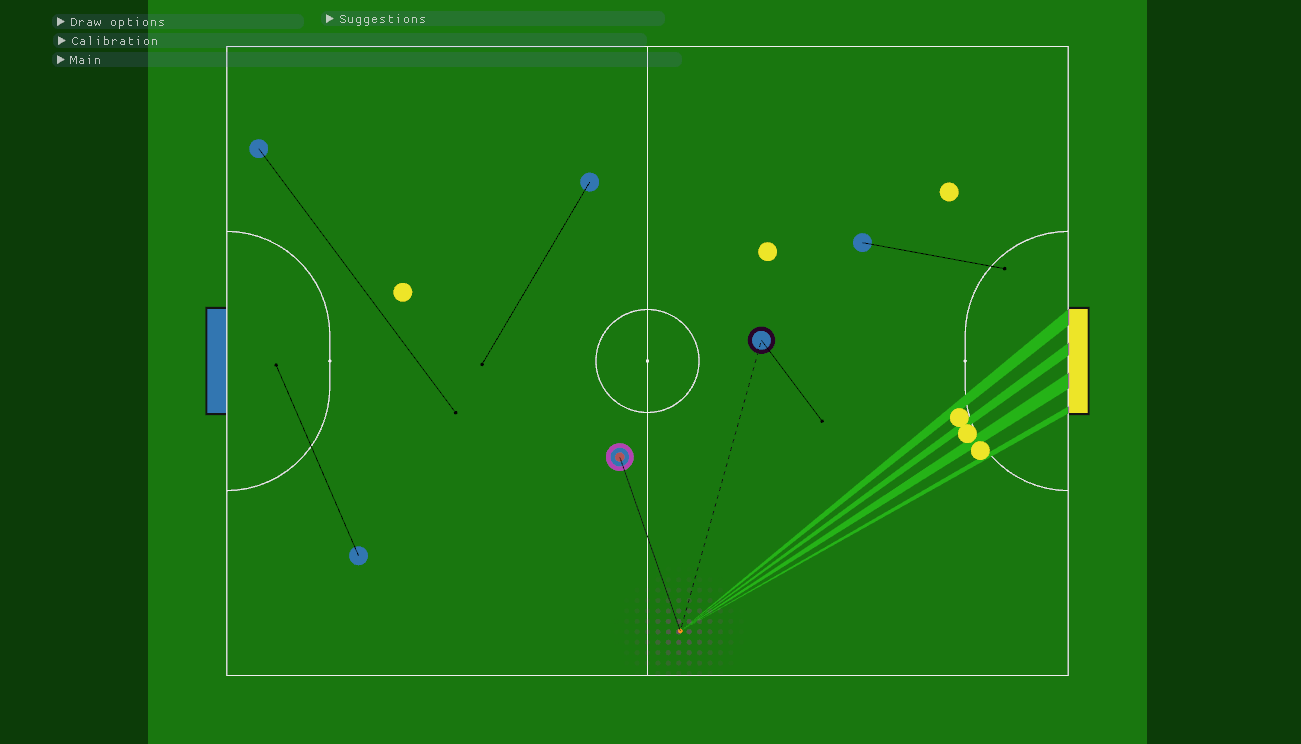
\includegraphics[width= 0.8\linewidth]{result/default_atq}
  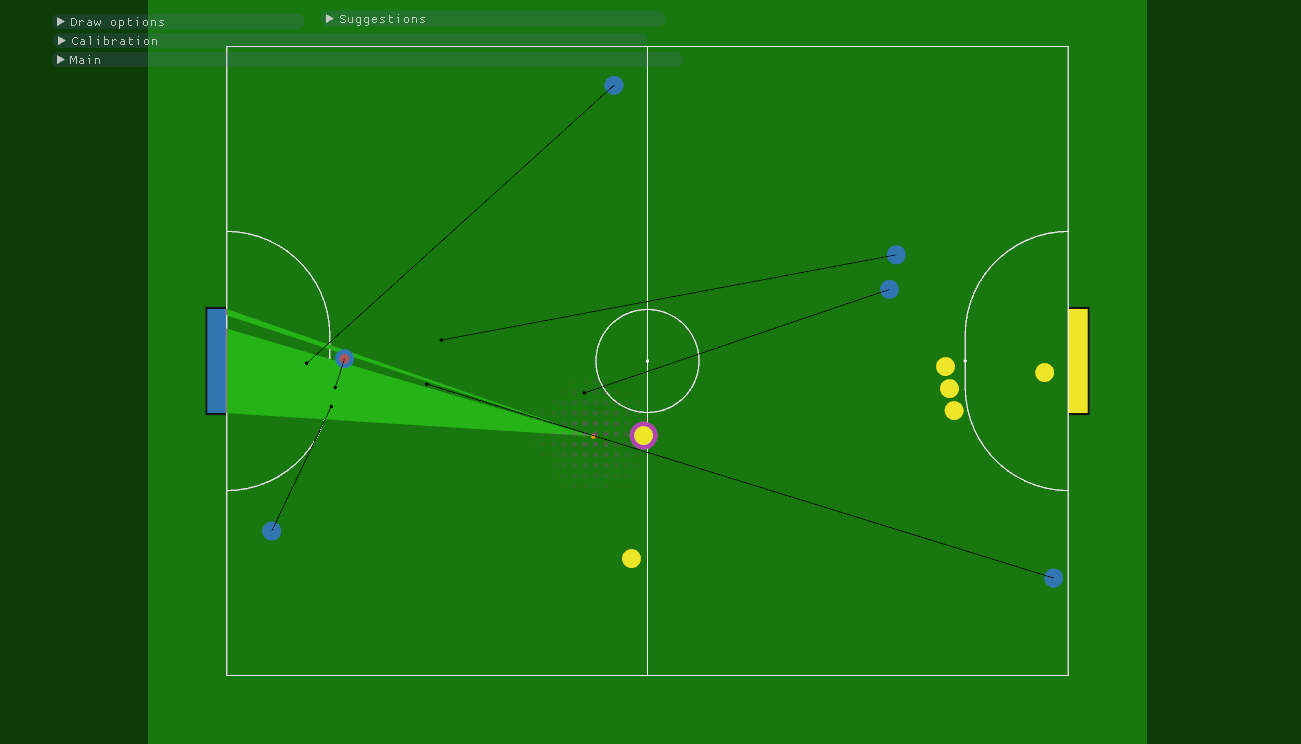
\includegraphics[width= 0.8\linewidth]{result/default_def}
  \caption{Planejamento com os parâmetros iniciais no
           ataque (acima) e na defesa (abaixo)}\label{fig:default}
\end{figure}


\section{Interface Gráfica}
